\section{Motivating Example}

Consider a safety monitoring device that is used to detect and report various hazardous condition in a critical care unit in a hospital. Among the several capabilities of the device, one of its requirement is to \emph{raise an alarm if the room temperature is more than 70 F for more than 5 minutes continuously}. In these systems, establishing traceability between the requirements to parts of the system that satisfy them is crucial to analyze and assess the impact of a change in either the requirements or the system on the other. Say, for this requirement, a trace link is established to a temperature sensor (\emph{measures the room temperature and reports the hazard if it is more than 70 F for more than 5 minutes continuously}) and, a LED (\emph{produces a blinking red light if the temperature sensor reports the hazard})- the two components that together satisfy the requirement. This trace helps identify which component get impacted by a change in the requirement. For instance, if there is a change in requirement to raise an alarm if the room temperature is more than 80 F (instead of 70 F), using the trace links established one could easily identify that the sensor functionality needs to be changed to meet the new requirement.
 
However, if there was an alternate way the previous requirement was satisfied, that was not explicitly traced, then the impact analysis to change only that sensor functionality is not adequate. If this device had two redundant sensors and different alarming components, say for fault tolerance, then the device might continue to raise an alarm when temperature is more than 70 F in-spite of the change to one of the sensors to measure 80 F. Also, it is common for a component to satisfy many requirements, such as the buzzer and LED that can alarm for other types of hazards. Capturing all the traces between the all the requirements will help bidirectionally assess the impact to the artifacts. Hence, without insight into the all the possible trace links between requirements and its realization, in our opinion, the results of analysis using traceability could be potentially inadequate and misleading. While we illustrate the problem of traceability with a toy example, in practice systems are complex with hundreds of system requirements and numerous components with potentially thousands of component requirements that may induce several ways to satisfy the requirements.  Unfortunately, neither the completeness of traceability nor its benefits are discussed in the existing literature.

\section{Formal Representation of Traceability}
\label{sec:motivation}
\newcommand{\satisfies}{\vdash_{\!\!s}}
\newcommand{\nsatisfies}{\nvdash_{\!\!s}}

In its simplest sense, traceability is capturing the relationship between artifacts. There are three building blocks for traceability - a \emph{source artifact} from which relationship should be established, \emph{the target artifact} to which the source artifact be related and the \emph{trace relationship}, that describes the association between the artifacts.  To provide notation, we write $T \vdash e$ to state that a set of target artifacts $T$ is sufficient to establish a traceability relationship $\vdash$ to source element $e$.
For requirements satisfaction traceability, the source artifacts are requirements $\Delta$, the target artifacts $\Sigma$ are the elements that realize the requirement such as lines of code, design elements, system or world assumptions, or lower-level requirements, and the trace relationship is \emph{satisfies}.  Thus, we write $S \satisfies r$ for $S \subseteq \Sigma$ and $r \in \Delta$ when set of target elements $S$ satisfies requirement $r$.  We will use $S, S'$ to denote sets of target elements and $r, r'$ to denote requirements.
%
%While the trace direction could be bidirectional, for now lets consider trace from requirements to its realization. In the next section we explain how this can be used to establish the other direction.
%
%Let $R$ denote the set of all requirements of the system %where $R = \{R_1, R_2...R_n\}$  and $R_{1...n}$ are individual requirements. Let
%and $I$ denote the set of all target artifacts. %where $I = \{I_1, I_2...I_m\}$ and $I_{1...m}$ denotes each target artifact.
%As mentioned earlier, the target artifact could be lines of source code, model elements (in model based development), assumptions etc. %\anitha{In the following whenever we use $r$ we mean it is a single requirement, $r \in R$.}
%A satisfaction argument establishes the validity of a requirement through a sufficient set of target artifacts. \anitha{am I saying the right thing?}. Formally it is represented as,
%
%$$ S \satisfies r $$
%$$ where~r \in R~and~S\subseteq I$$
%
We assume that the satisfaction deduction $\satisfies$ is monotonic on the subset relation over $\Sigma$, that is, if $S \subset S'$ and $S \satisfies r$, then $S' \satisfies r$.

%$$ (S'\subseteq I~and~S \subset S' ~and~ S \satisfies r) \implies S' \satisfies r$$

%We assume that satisfaction argument is monotonic on I, that is: $(S_x \subset S_y \land S_x \satisfies R_x) \implies S_y \satisfies R_x$.
%, $R_x$, establishes, $S_x \satisfies Rx$, where $S_x = \{I_1, I_2,... I_k\}$, the elements of the target artifact that together satisfy the requirement.

%A \emph{requirement satisfaction trace (RST)} is the relation between a requirement and the set of target artifacts that establish the satisfaction of the requirements.  %While traditional way of establishing a trace concerns relating a requirement to a target artifact, the requirements satisfaction trace relates the requirement to a set of target artifacts that can demonstrate the satisfaction of requirements, thus establish a sematic basis for the traceability.

%$$ RST: \Delta \times 2^{\Sigma}$$
%where $$ RST(r, S) \equiv S \satisfies r $$

%\anitha{I know I asked this before, but just to confirm, is it enough that we mentioned that we assume monotonicity earlier in this section; but somehow it reads as if we discuss about it only in that context of satisfaction argument?}
%\anitha{$$ \forall i \in I \cdot S \cup i \satisfies r) $$}

%\mike{I'm renaming $RST_{m}$ the set of support $SOS$; the fewer terms, the better }

The monotonicity of the satisfaction relation means that, unless {\em all} elements of the implementation $\Sigma$ are required for a proof, there are multiple implementation sets $S \subset S' \subset \ldots \subset \Sigma$ that can satisfy a given requirement $r$.  However, we are primarily interested in {\em minimal} sets that satisfy $r$; tracing a requirement to the entire implementation is not particularly enlightening!  We call a minimal set of target artifacts the \emph{set of support} for that requirement, and define the $SOS$ relation to associate sets of support to requirements.

$$ \ SOS(r, S) \equiv S \satisfies r~\land (\forall S'\ .\ S' \subset S \implies S' \nsatisfies r) $$

$SOS$ maps sets of support to a requirement. As mentioned earlier, there could be many sets of support for a requirement. To capture that notion, we define, \emph{all sets of support ($ASOS$)} for a requirement as an association to all its sets of support.

$$ ASOS(r) : \{\ S | (r,S) \in SOS(r,S)\ \} $$

The set of $ASOS$-es for all requirements represents the complete traceability of the system.

%The $ASOS$ for a requirement can be envisioned as a matrix in which each row represents a target artifact in $\Sigma$, each column represents a set of support for requirement $r$, and cells contain an 'x' if the target artifact is used in the set of support and is otherwise blank.\mike{Does this really aid explanation?}
%
%The set of $ASOS$-es for all requirements represents the complete traceability of the system. One can envision this as a 3 dimensional traceability matrix, where the third dimension is each requirement.\mike{again, is this helpful?}


%$$ CRST_m: r \longrightarrow \mathfrak{S}$$
%$$ where~~r \in R~and~\mathfrak{S} = \bigcup(S)$$
%$$ \forall e \in \mathfrak{S} \cdot e \satisfies r ~and~ \not \exists e'\subseteq I ~and~e'\notin \mathfrak{S}~and~ e' \satisfies r $$

%as $\Sigma_{mx} = \{S_{xm1}, S_{xm2}....S_{xmk}\}$ where each $S_{xk} \satisfies R_x$. Similarly, the \emph{complete minimal requirements satisfaction traces} for all requirements for the system is represented as \anitha{can i union tuples?}  $$\bigcup_{\forall x, (R_x \in R)} (R_x, \Sigma_{mx}, \satisfies)$$

%
%While $RST_m$ maps one set of support to a requirement, as mentioned earlier, there could be many sets of support for a requirement. To capture that notion, we define, \emph{complete minimal requirement satisfaction trace} for a requirement $R_x$, can be represented as $\Sigma_{mx} = \{S_{xm1}, S_{xm2}....S_{xmk}\}$ where each $S_{xk} \satisfies R_x$. Similarly, the \emph{complete minimal requirements satisfaction traces} for all requirements for the system is represented as \anitha{can i union tuples?}  $$\bigcup_{\forall x, (R_x \in R)} (R_x, \Sigma_{mx}, \satisfies)$$
%
%
% %
%
% While the traditional way of establishing a trace concerns relating a requirement to a target artifact, the requirements satisfaction trace relates a group of target artifacts to a requirement that together (formally conjunction) satisfy the requirements.
%
% such that I_1 \wedge I_2 \wedge... I_k are the elements of the target artifact that are necessary to satisfy the requirement. The term ``necessary" elements means that removing one of them from $S_x$ invalidates the satisfaction argument. Formally, $\forall j (S_x\setminus{I_j} \nvdash R_x)$ where $(I_j \in S_x)$. We call such an $S_x$ as a \emph{set of support} for the requirement $R_x$.

% that can be derived from a satisfaction argument can be represented a tuple (R_i, S_i, $\satisfies$), where $R_i$ denotes a requirement (the source artifact), $S_i$ is a set of support for $R_i$ and the $\satisfies$ is the relationship between the two. Although it may seem unnecessary to include the relationship in the tuple, since we call it the "satisfaction" trace, explicitly stating it ensures that the rationale for the trace is neither lost nor mis-interpreted. While the traditional way of establishing is trace concerns a requirement and an element in the target artifact, the requirements satisfaction trace relates a group of target artifact elements to a requirement that together (formally conjunction) and "only" if they are together will satisfy the requirements.


%\anitha{Explains SA and traceability - formally definitions of each requiremnt, each entitiy of trace artifact, set of support, trace link, traditional requirements traceability and  one requirements satsifaction traceability and all RST}
%
%
%Intuitively, traceability is a bookkeeping activity; it is about explicitly capturing the relationship between entities of artifacts so that one can perform some form of analysis about them. While engineering systems, the ability to trace a requirement, particulary functional requirements, to artifacts that were created by to satisfy them such as design, implementation etc, we will refer to them as \emph{target artifact}, has been very useful for several types of analysis. Some of them include~\cite{rich
 traceability paper} :
%\begin{itemize}
%  \item \textbf{Impact analysis} that helps understand how a change in the requirement change will affect the other artifacts; determine how and where the requirements are realized in the associated artifact; and, assess if all requirements are realized in the artifacts.
%  \item \textbf{Dependency analysis}, the opposite of impact analysis, that helps identify the requirements that influenced the creation of the other artifact; analyse which requirement's satisfaction will be affected if there is a change in the artifact; and determine if there are entities with the artifact that do not trace to any requirement that in turn helps measure the coverage of requirements over the artifact.
%\end{itemize}
%
%Unfortunately, it was found that merely relating functional requirements to other artifacts, without a documentation of the rationale for why and how they were related, was often to be inadequate to perform useful analysis in practice~\cite{Trace links explained: An automated approach for generating rationales}. Further, validation of the established relationships is also a challenging task. In that context, \textbf{\emph{Satisfaction Arguments}} provide a meaningful way to establish traceability between functional requirements and its realization. Originally proposed by Zave and Jackson, satisfaction argument is an approach to demonstrate how the behaviors of the system along with the assumptions made about its environment satisfy the functional requirements. This approach significantly the usual way traceability was thought. First, it established a semantic rationale for traceability, ``satisfied by" relationship between the requirements and the target artifact. Second, it illuminated that tracing to just one target artifact may not be sufficient to establish the relationship; in particular, it traced to both the environmental assumptions as well as the description of the system that together satisfies the requirements. Although it was restricted to one specific type of relationship for tracing, it resulted in precise impact and dependency analysis.
%
%While satisfaction arguments help establish a sematic trace link between requirements and target artifacts, it is unclear if one should capture one or all such satisfaction arguments. For instance, in safety critical system domain, for fault tolerance one could intentionally add multiple ways to satisfy a requirement or one could unintentionally add system functionality that leads to multiple ways of satisfying a requirement. From a system assurance perspective (the original intent of the satisfaction arguments) it may be sufficient to identify one of them, but from a traceability perspective it may just be ``a" trace link. This raises a fundamental question, nor just about requirements traceability, but traceability in general \emph{Should one establish one or all trace links between artifacts?}
%
%Let us illustrate this with an small example. Consider a safety device whose requirement is to \emph{raise an alarm if hazard occurs}. The device is composed of two redundant sensors (for fault tolerance) whose requirement is to \emph{detect and report if a hazard occurs} and a buzzer that \emph{sounds an audible alarm if either one of sensors report a hazard}; \emph{the buzzer shall otherwise remain silent}. Since the sensors are redundant, to establish that the system level requirements are satisfied, one of the sensors and the buzzer is sufficient. Using the SA approach to document traceability, it may appear sufficient to capture trace links between the requirements and that sensor and the buzzer. However, an astute reader might question about the alternate SA that involves the other sensor and buzzer. This is exactly our question too. Currently, it is unclear whether one should establish one or all trace links between artifacts.
%
%In our opinion, to completely realize the benefits of traceability, one should capture all the trace links between artifacts. For instance, if one intends to change the requirements of one of the sensors then the fact that the satisfaction of the system requirement is unaffected is not visible unless the complete traceability was recorded. While we illustrated with a toy example, in practice systems are complex with hundreds of system requirements and numerous components with potentially thousands of component requirements, that makes establishing complete traceability crucial to perform meticulous analysis. Unfortunately, neither the completeness of traceability nor its benefits are not well discussed in the existing literature. In the following section, we elaborate the need to establish complete traceability.

%
%By recording all possible ways the requirements can be satisfied, one can identify those component that do not contribute to any system requirement. This helps assess the completeness of system requirements in capturing all the behaviors induced by its components.
%
%While the above was a toy example, in practice systems are complex with hundreds of system requirements and numerous components with potentially thousands of component requirements, that makes manual traceability infeasible. In fact, this is particularly an issue in model based developments where with increase in complexity of the models, it becomes practically infeasible to either manually add or capture all trace links. Hence, what we need is an approach that can automatically and efficiently establish all trace links between the requirements and parts of model that satisfy then.


%
%AGREE uses JKind, a bounded model checker, to verify the requirements of the system. Model checking is a technique that allows reasoning whether the requirements expressed using temporal logic notion are satisfied by the model of the system. Given the model of the system and its requirements, AGREE and JKind transforms the model into a logical formula that defines how the system can evolve from one time instant to the next time instant, starting from an initial state. This transformed logical formula provides the structure for the model checker to prove the requirements of the system using the principle of mathematical induction. If the model checker finds a violation of the requirement it reports a counter example, otherwise declares that the requirement is valid.
%
%While the compositional verification was very useful in proving system level requirements, in the event that requirement is proved, it is not always clear what level of assurance should be invested in the result.  Given that these kinds of analyses are typically performed for safety critical system, this can lead to overconfidence in the behavior of the fielded system. It is well known that issues such as vacuity~\cite{Kupferman03:Vacuity} can cause verification to succeed despite errors in a requirements or in the model. Even for non-vacuous requirements, it is possible to over-constrain the {\em environment} of the model such that the implementation will not work in the actual operating environment. Hence, to gain confidence over the verification we pursed an approach that would provide us with an evidence of the successful verification. An evidence in this context is nothing but an explanation about which parts of the model (the component requirements and system assumptions) the model checker used to prove the system level requirement.
%
%\begin{figure}[htb]
%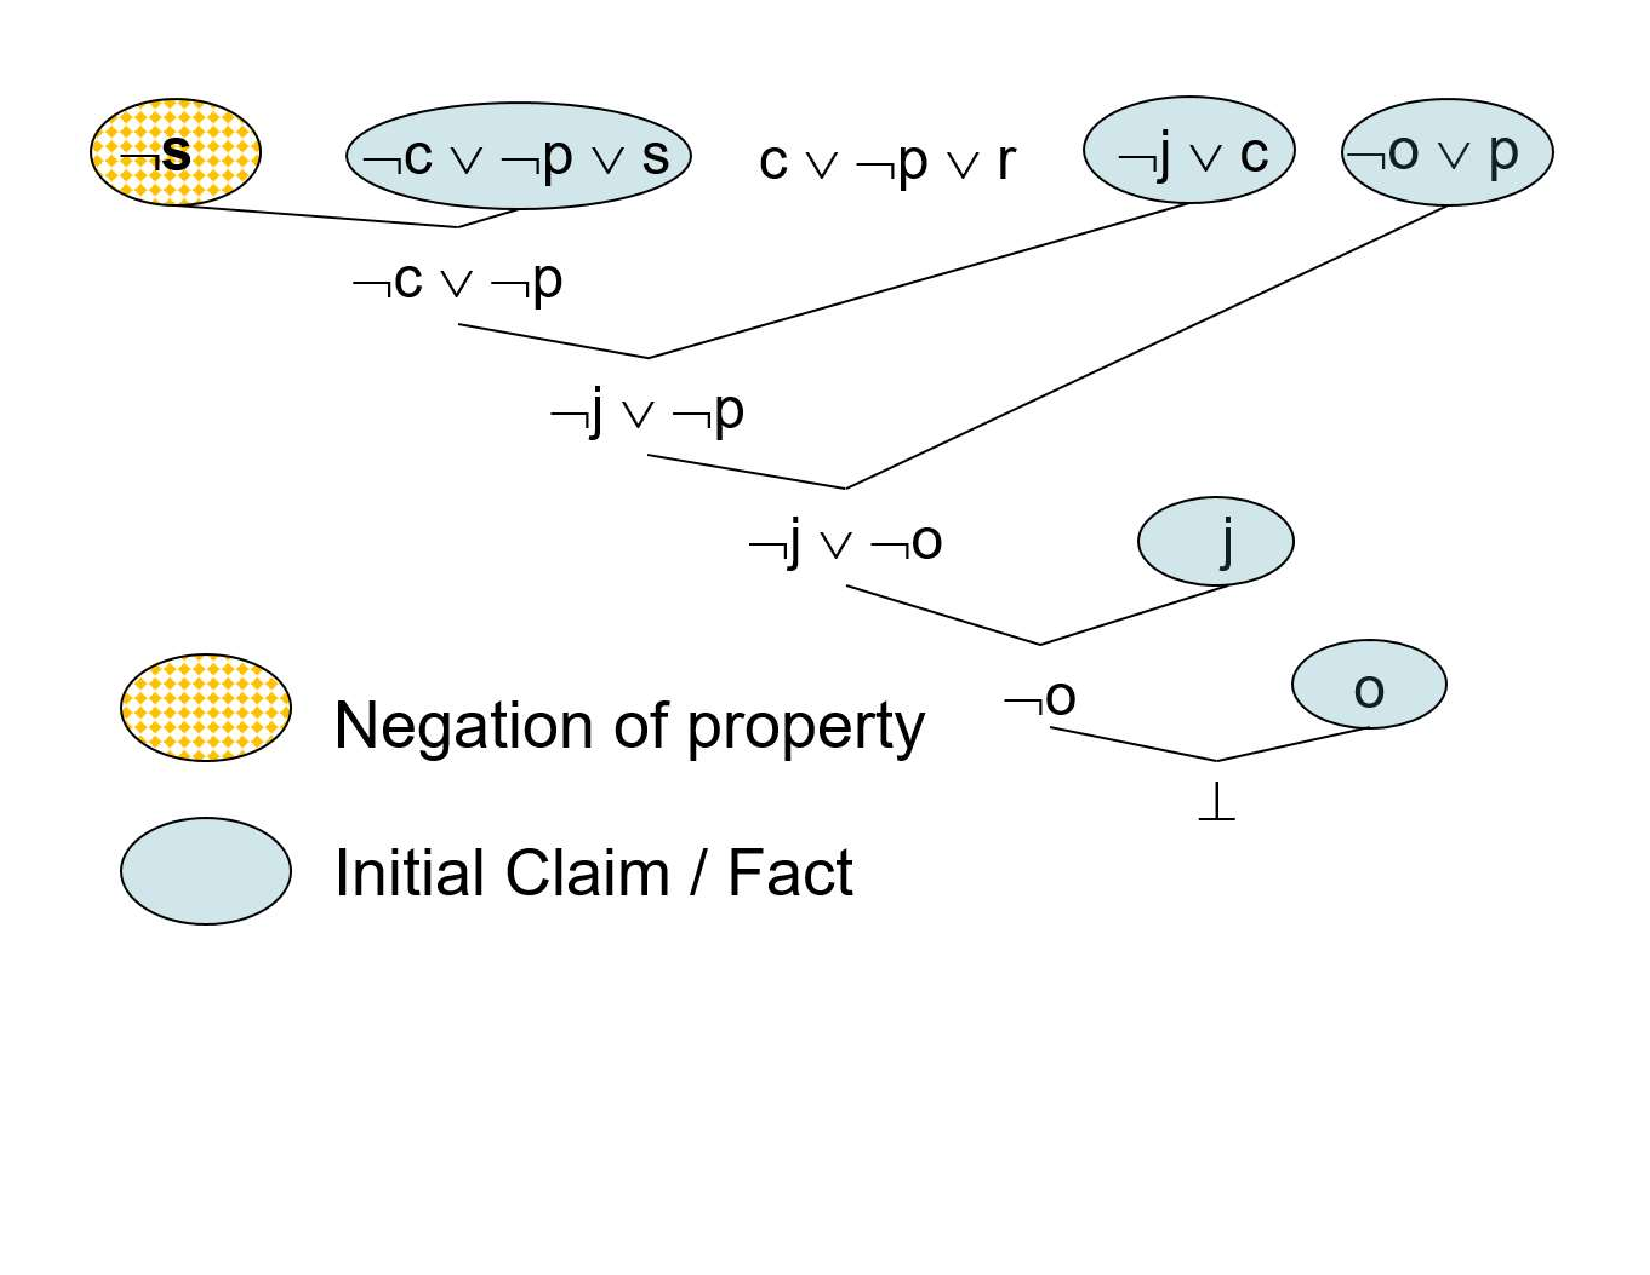
\includegraphics[width=\columnwidth]{images/proof.pdf}
%\caption{I will put a nicer picture}\label{fig:proof}
%\end{figure}
%
%To verify a requirement with respect to a model, SAT based model checkers like JKind, automatically constructs proofs of satisfaction. A proof can be visualized as a derivation tree where the leaves of the tree are axioms -- elements of the model such as components requirements, system assumptions -- and each interior node represents the application of an inference rule that leads to the claim, as shown in the Figure~\ref{fig:proof}. Our interest is to come up with an approach that will help extract the axioms that were necessary for the proof such that we can establish traceability to the requirements.
%
%While the proof generated by model checkers are typically invisible, SAT based model checkers allow users to query which axioms were used as part of the proof. We call the result to such a query, {\em inductive validity core} (IVC). The IVC helps explain how the solver reported the satisfaction of the requirement, that is comparable to the counterexample explains the negative result. In a recent work, we proposed a generic and efficient mechanism to extract the IVC from the proofs of requirements using inductive techniques. In general, the IVC extracted is not guaranteed to be contain only the necessary axioms, depending on how the model checker constructed the proof. Hence, in our approach after extracting the IVC we minimize it by recursively reducing them and checking if the remaining axioms are the necessary elements for the proof. Further, when induction is involved, many requirements are not themselves inductively provable and hence proof techniques introduce lemmas as part of the solving process in order to strengthen those requirements and make them inductive. The novelty of our approach is its efficient, accurate, and precise extraction of a minimum IVC in the presence of such auxiliary lemmas.
%
%In the next section we explain our approach to using the IVC to establish traceability between the requirements and actual parts of the model in a way that is useful to the user.



%
%
%
%
%Our aim is to establish requirements traceability by leveraging the capability of the sophisticated model based tools. \anitha{editing.....}
%
%
%However, with the increase in the size and complexity of the models, it is not easy to understand how and where the requirements are implemented in the models.
%
%
%Such as an association between the requirements and the model, in other words traceability, helps effectively perform :
%\begin{itemize}
%  \item \textbf{Impact analysis} - To determine which parts of the model implements the requirement, how a change in requirement affects the model and check if all requirements are implemented by its components.
%  \item \textbf{Dependency analysis} -  To identify which requirement had given rise to specific parts of the model, identify which requirement will be affected if the component is changed, assess the coverage of the requirements over the model, determine which parts of the components do not trace to any requirement.
%\end{itemize}
%
%
%
%Our interest is to be able to establish requirements traceability in the context of model based development (MBD), in which the systems are modeled using some form of mathematical notations. MBD is emerging as a widely accepted technique to developing systems, especially safety critical systems and has been very successful in identifying errors early in the development cycle and help improve the quality of the system.
%
%
%
%\textbf{Existing MBD traceability techniques.}Unfortunately, one of the major challenges in MDB is precisely that traceability. The main reason behind the difficulty is the inherent complexity of the models that makes the process of manually establishing trace links exhausting. However, there has been some research efforts to automatically establish the traceability between requirements and model elements. Some of them include :
%\begin{itemize}
%  \item Event-Based Traceability (EBT) (Cleland-Huang et al) is a method that automatically establishes trace links and maintains it, between requirements to models, using event-based mechanisms.
%  \item Egyed and Grunbacher enhance the basis from which they derive links by following the approach of dynamic program analysis: They record program execution traces (these are—as described earlier—dynamic program behavior logs) from the execution of test-cases. They combine the results with a set of requirements-to-code traceability links, which have to be established manually beforehand and infer traceability links between requirements.
%  \item Wenzel et al. describe a tool which is able to compare the version history of models, to derive traceability links, and consequently, to reconstruct the evolution steps of single model elements.
%  \item I have a survey paper, I will fill more relevant work here
%\end{itemize}
%
%\textbf{SA is good technique for traceability.}While the above techniques establish trace links, without a sematic rationale, Satisfaction Arguments offer a meaningful way to establish traceability between functional requirements and its realization. Unlike traditional traceability that just links two artifacts, satisfaction arguments are aimed to provide an explanation to why the traceability was established. It has been recognised that establishing traceability using satisfaction arguments has been very useful.\anitha{I want to make this a single sentence to lead to our work.}
%
%
%
%
%
%\textbf{In previous work we} demonstrated an approach to system construction in which compositional proofs are used to to establish satisfaction arguments. Given an architectural model of the system (decomposition of system into components) in which each component (including the system) is endowed with its own behavioral requirements and assumptions it makes about its environment, our approach compositionally verifies if system level requirements as a logical consequence of the component level requirements. To implement our approach, we used a tool called AGREE \cite{NFM2012:CoGaMiWhLaLu} -- a compositional reasoning framework based on assume-guarantee reasoning ~\cite{McMillan99:circ}, that provides an appropriate mechanism for formally capturing the model of the system and verify system requirements.

